\section{workflow}


%------------------------------------------------
\begin{frame}[fragile]{流程}

需要如下步骤:
\begin{itemize}
\item 确保手机可以进入fastboot.
\item 替换刷入boot\_img\_for\_dw7914\_test.img 并使手机开机,出现adb 口。
\item 进入adb shell .执行 测试命令。
\end{itemize}

接下来是详细流程。

\end{frame}


%------------------------------------------------
\begin{frame}[fragile]{进入fastboot 方法一}

 有两种方式进入fastboot,
\begin{itemize}
  \item 手机可以开机的情况下 使用 adb 命令
  \item   使用 fastboot oem alive
\end{itemize}


 当你 可以让手机开机 的时候:

手机开机,使用USB 线 连接电脑,进入windows设备管理器看看有没有adb 口,如下红线部分的字样:
\begin{figure}[htbp]
\begin{center}
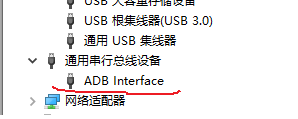
\includegraphics[width=5cm]{img/adb}
\caption{adb interface }
\label{adb interface}
\end{center}
\vspace{-0.5em}
\end{figure}

\end{frame}


%------------------------------------------------
\begin{frame}[fragile]{确保手机可以进入fastboot}

如果有,使用windows 命令行输入如下命令后 按下 Enter 键:
  \begin{lstlisting}
  adb reboot bootloader
  \end{lstlisting}
  \begin{figure}[htbp]
  \begin{center}
  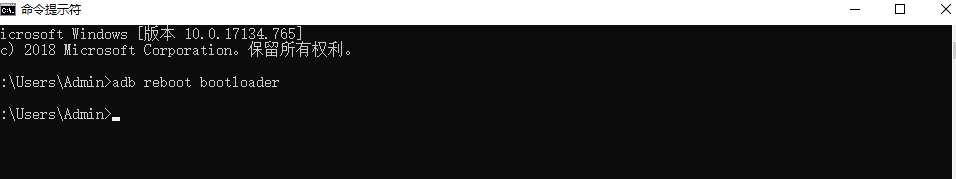
\includegraphics[width=10cm]{img/rebootbootloader}
  \caption{adb cmd}
  \label{adb cmd}
  \end{center}
  \vspace{-0.5em}
  \end{figure}

此时 板子/手机 已经在fastboot 模式了。

\end{frame}




%------------------------------------------------
\begin{frame}[fragile]{替换镜像}

接下来在 将以下命令 中 最后一项的路径更改为你的路径,确保输入无误后,按下回车执行。
  \begin{lstlisting}
  fastboot flash boot C:\Users\Admin\Desktop\DW7914_TEST\boot_img_for_dw7914_test.img
  \end{lstlisting}
这里路径不能复制粘贴,请使用 您本地路径。

执行结果无误的话应该会是这个样子:
  \begin{figure}[htbp]
  \begin{center}
  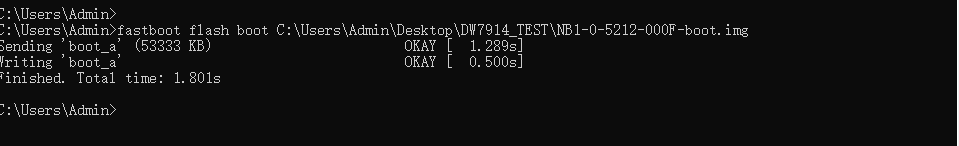
\includegraphics[width=10cm]{img/replace}
  \caption{adb cmd replace}
  \label{adb cmd replace}
  \end{center}
  \vspace{-0.5em}
  \end{figure}

此时 板子/手机 中的 boot 分区已经被替换为新的 boot 内容。但是板子/手机还是在 fastboot 模式。

\end{frame}



%------------------------------------------------
\begin{frame}[fragile]{reboot}

紧接着上一步,执行
  \begin{lstlisting}
  fastboot reboot
  \end{lstlisting}
使手机重启。然后等待 出现adb 口。


  \begin{figure}[htbp]
  \begin{center}
  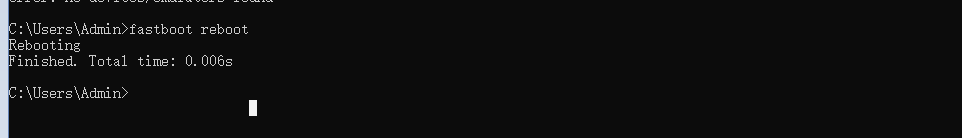
\includegraphics[width=10cm]{img/reboot}
  \caption{adb cmd reboot}
  \label{adb cmd reboot}
  \end{center}
  \vspace{-0.5em}
  \end{figure}

这个时候 板子会重启,应用刚才的变化。

\end{frame}




%------------------------------------------------
\begin{frame}[fragile]{adb shell}

等待板子启动后, 出现 adb 口,执行
  \begin{lstlisting}
  adb shell
  \end{lstlisting}
进入adb shell:


  \begin{figure}[htbp]
  \begin{center}
  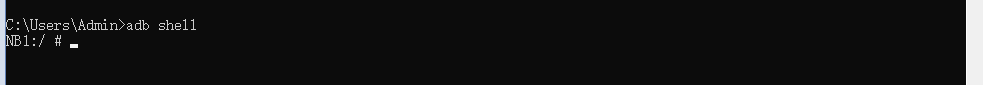
\includegraphics[width=10cm]{img/shell}
  \caption{adb cmd shell}
  \label{adb cmd shell}
  \end{center}
  \vspace{-0.5em}
  \end{figure}

\end{frame}


%------------------------------------------------
\begin{frame}[fragile]{操作节点 完成测试}

在adb shell  中 输入以下命令 :
  \begin{lstlisting}
  echo  1 > /sys/class/leds/vibrator/go
  \end{lstlisting}
按下Enter 使执行,同时产生震动。

如果使用的复制粘贴 注意看有没有空格,有的话请手动消除。

  \begin{figure}[htbp]
  \begin{center}
  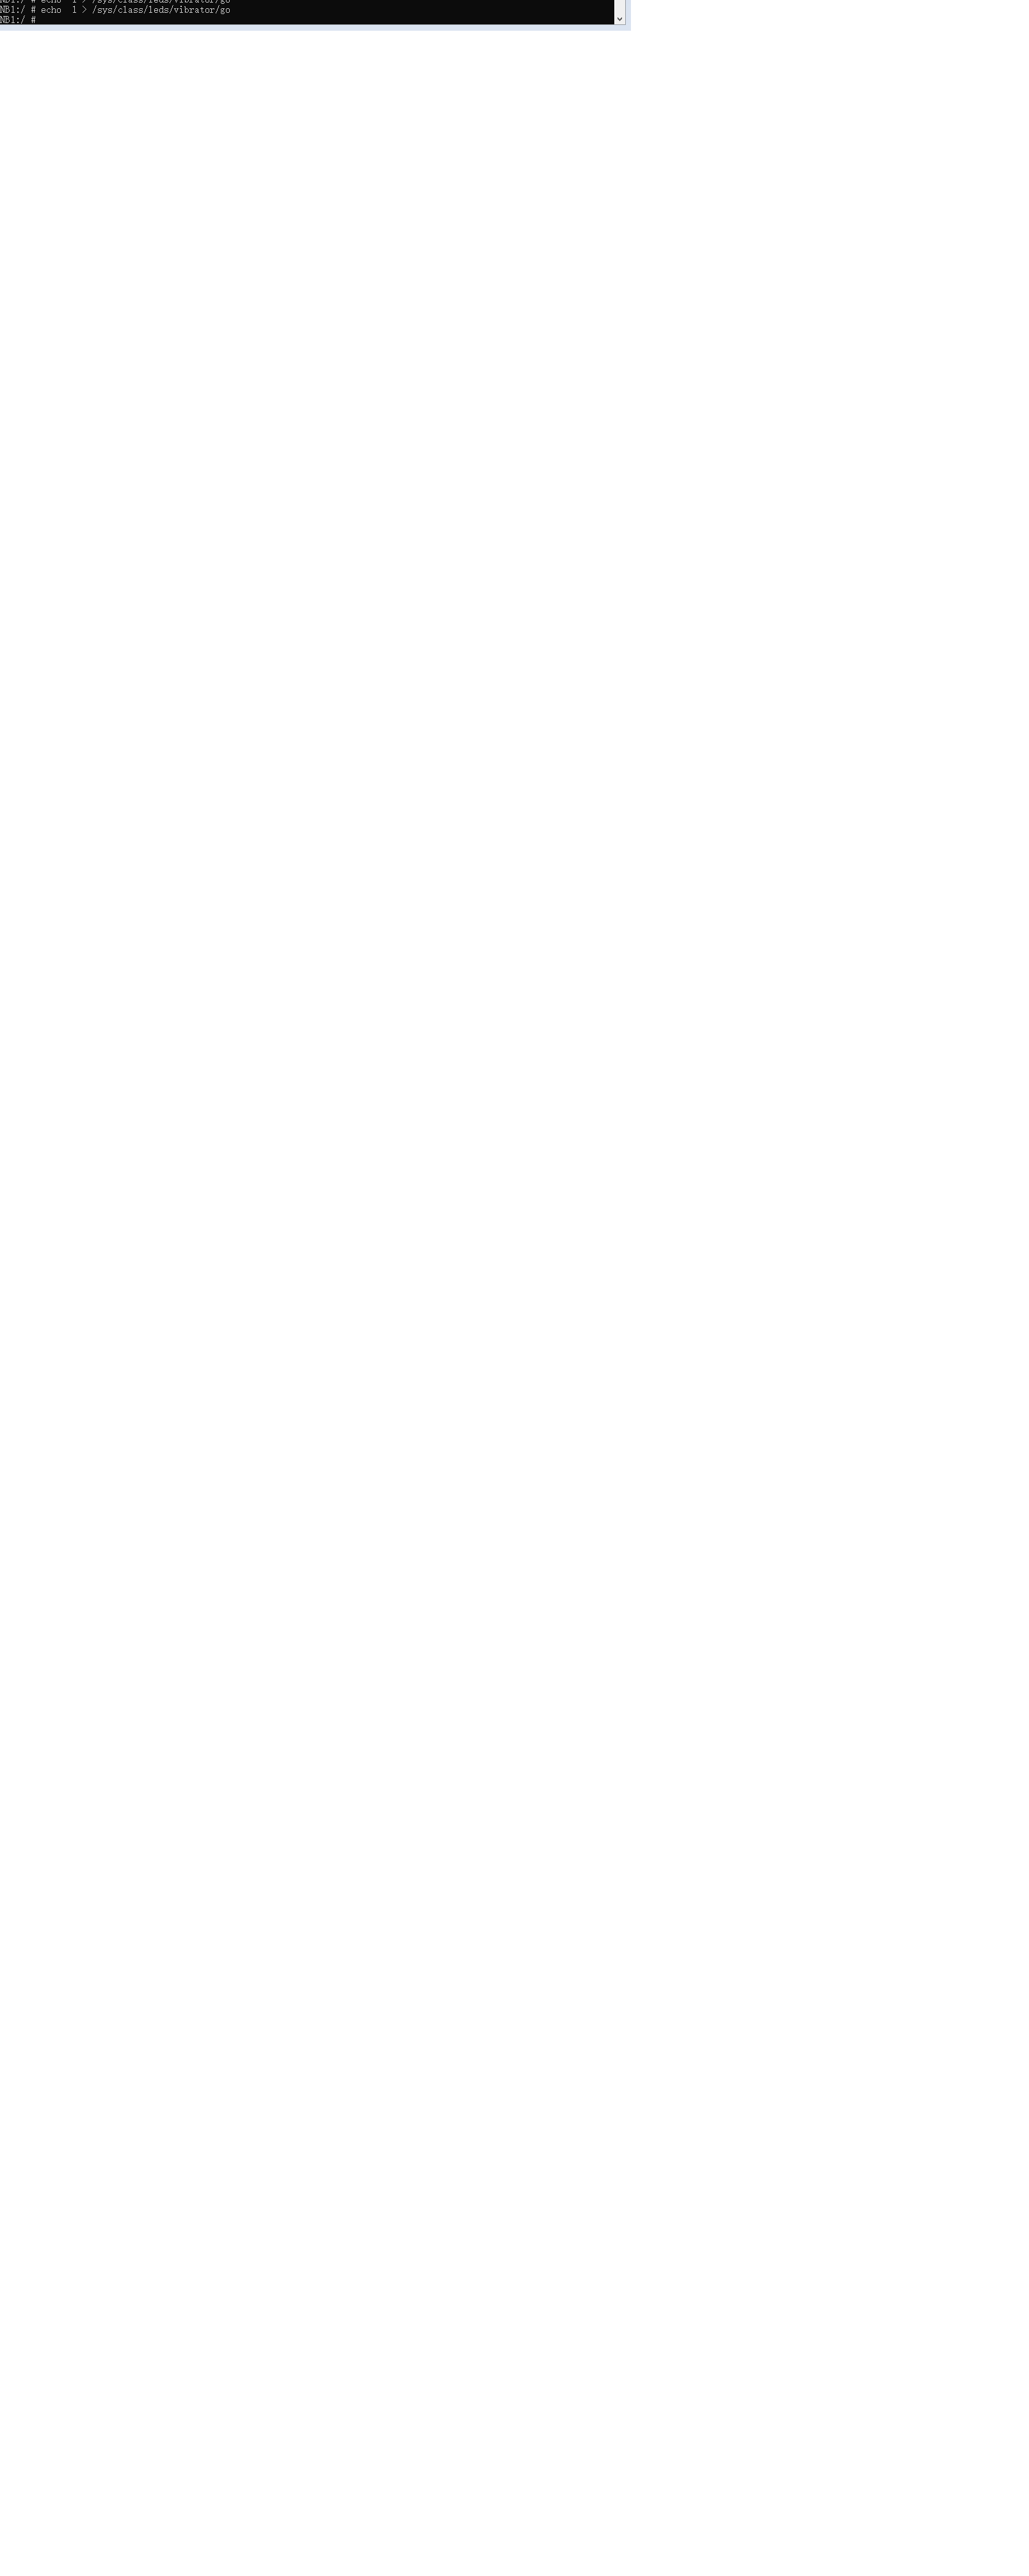
\includegraphics[width=15cm]{img/go}
  \caption{adb cmd shell go}
  \label{adb cmd shell go}
  \end{center}
  \vspace{-0.5em}
  \end{figure}

\end{frame}


%------------------------------------------------
\begin{frame}[fragile]{操作节点 完成测试}

在上个步骤中,每执行一次如下命令;
\begin{lstlisting}
echo  1 > /sys/class/leds/vibrator/go
\end{lstlisting}
都会使dw7914 驱动马达震动。








至此 测试结束,谢谢帮助!

\end{frame}
